\documentclass{article}
\usepackage[final]{neurips_2024}
\usepackage[T1]{fontenc}    
\usepackage{hyperref}       
\usepackage{url}            
\usepackage{booktabs}       
\usepackage{amsfonts}       
\usepackage{nicefrac}       
\usepackage{microtype}      
\usepackage{xcolor}         
\usepackage{graphicx}   
\usepackage{amsmath}
\usepackage{float}

\setcitestyle{numbers}

\title{COMP 579 Final Project Report: Reinforcement Learning for Ms. Pac-Man}

\author{
    Ivy Hu\textsuperscript{1} \quad
    Simon Li\textsuperscript{2} \quad
    Kenza Bellebouir\textsuperscript{1} \\
    \texttt{nanqing.hu@mail.mcgill.ca} \quad
    \texttt{xi.yang.li@mcgill.ca} \quad
    \texttt{kenza.bellebouir@mail.mcgill.ca} \\
    \textsuperscript{1}Department of Computer Science, McGill University \\
    \textsuperscript{2}Department of Electrical Engineering, McGill University
}

\begin{document}

\maketitle

\begin{abstract}
  We investigate the comparative performance of Rainbow DQN and Proximal Policy Optimization (PPO) in the visually complex Ms. Pac-Man environment. Our study evaluates learning dynamics, hyperparameter sensitivity, and robustness to visual perturbations. Rainbow DQN consistently achieves higher peak rewards and demonstrates stronger long-term learning, while PPO shows faster early convergence but suffers from instability. We also conduct ablation studies and color-based generalization tests, offering practical insights into the role of architecture and training design in sparse-reward, high-variance domains.
\end{abstract}

\section{Introduction}

Deep reinforcement learning (RL) has achieved notable success in high-dimensional decision-making tasks, particularly within the Arcade Learning Environment (ALE) \cite{ale}, which provides a unified platform for evaluating algorithms on Atari 2600 games \cite{mnih2015human}. These environments are characterized by partial observability, sparse and delayed rewards, and the need for both short-term reactivity and long-term planning.

Among them, \textit{Ms. Pac-Man} is a particularly challenging domain due to its stochastic dynamics, diverse strategic possibilities, and visually rich inputs. It is thus well-suited for evaluating algorithmic robustness and scalability. In this work, we compare two prominent deep RL methods: Rainbow DQN \cite{hessel2018rainbow}, an enhanced value-based agent that integrates six key improvements over DQN, and Proximal Policy Optimization (PPO) \cite{schulman2017proximal}, a widely used policy-gradient algorithm known for its simplicity and stability.

We implement both agents in the \texttt{MsPacman-v0} environment and conduct a detailed empirical evaluation. Beyond comparing baseline performance, we perform an ablation study of Rainbow DQN to assess the contribution of prioritized experience replay, noisy networks, and multi-step returns. To evaluate generalization, we test trained agents under visual domain shifts introduced via color perturbations. We further analyze sensitivity to hyperparameters by conducting targeted sweeps to identify configurations yielding strong and stable performance.

This study provides insights into the design and evaluation of RL algorithms in complex visual settings, highlighting the internal dynamics and generalization capabilities of Rainbow DQN relative to PPO.

\section{Background}

\subsection{Reinforcement Learning and MDPs}

Reinforcement Learning formalizes sequential decision-making as a Markov Decision Process (MDP), defined by $(\mathcal{S}, \mathcal{A}, \mathcal{P}, \mathcal{R}, \gamma)$, where $\mathcal{S}$ is the state space, $\mathcal{A}$ the action space, $\mathcal{P}(s'|s,a)$ the transition model, $\mathcal{R}(s,a)$ the reward function, and $\gamma \in [0,1)$ the discount factor. The agent selects actions to maximize expected return $\mathbb{E}[\sum_t \gamma^t r_t]$ based on its interactions with the environment.

\subsection{The Ms. Pac-Man Environment}

The \texttt{MsPacman-v0} environment is a high-dimensional, partially observable MDP. Each observation is a $210 \times 160 \times 3$ RGB frame, preprocessed to $84 \times 84$ grayscale. The action space consists of discrete directional commands and a no-op. Reward signals are sparse, with +10 for pellets, +200 for ghosts after consuming a power pellet, and a time-step penalty of –1. An episode ends when the agent loses three lives.

This environment presents multiple challenges: pixel-based observations limit access to the full game state, ghost behavior is stochastic and partially unpredictable, and the sparse reward structure complicates credit assignment and learning signal propagation. Additionally, the lack of intermediate rewards increases the difficulty of learning effective threat avoidance or path planning strategies.

\subsection{Rainbow DQN}

Rainbow DQN \cite{hessel2018rainbow} combines several enhancements to the original DQN \cite{mnih2015human}, aiming to improve sample efficiency, stability, and exploration. Double Q-learning addresses overestimation bias by decoupling action selection and evaluation in target computation. The dueling network architecture separates state-value and advantage estimation to refine action selection. Prioritized experience replay focuses learning on high-error transitions, improving data efficiency. Noisy networks inject trainable stochasticity into parameters, facilitating more efficient exploration. Multi-step returns accelerate learning by propagating rewards over multiple future steps. Distributional RL (C51) models a categorical distribution over future returns, enabling richer value representation.

\subsection{Proximal Policy Optimization (PPO)}

PPO \cite{schulman2017proximal} is a first-order policy-gradient algorithm that improves training stability by limiting policy updates through a clipped surrogate objective:
\[
L^{\text{CLIP}}(\theta) = \mathbb{E}_t \left[ \min \left( r_t(\theta) \hat{A}_t, \text{clip}(r_t(\theta), 1 - \epsilon, 1 + \epsilon) \hat{A}_t \right) \right],
\]
where $r_t(\theta)$ is the probability ratio between the new and old policies, and $\hat{A}_t$ is an estimate of the advantage function. PPO strikes a balance between exploration and stability, making it suitable for a wide range of tasks without extensive tuning.

\subsection{Evaluation Challenges}

Evaluating agents in visually rich environments like Ms. Pac-Man is non-trivial. RL training is often unstable due to non-stationarity, bootstrapping errors, and high sensitivity to hyperparameters. Sample efficiency is critical, especially when training from pixel inputs requires millions of frames. Generalization remains an open challenge, as agents frequently overfit to the visual statistics of the training domain. Even minor pixel-level perturbations can lead to catastrophic performance drops, as shown in \cite{zhang2020investigation}.

\subsection{Related Work}

Prior approaches to Ms. Pac-Man have explored architectural and algorithmic enhancements. Toromanoff et al. \cite{toromanoff2019deep} combined CNNs with recurrent networks to mitigate partial observability, achieving performance significantly better than DQN. Other works, such as Pieters et al. \cite{pieters2016monte}, introduced planning-based methods like Monte Carlo Tree Search for improved control, though these typically rely on engineered features. In contrast, we adopt a pure pixel-based learning paradigm and extend the robustness analysis by introducing controlled visual perturbations during evaluation.

\section{Methodology}

\subsection{Environment}

We evaluate agents in the \texttt{MsPacman-v0} environment from OpenAI Gym, based on the Arcade Learning Environment (ALE) \cite{ale}. The environment outputs raw $210 \times 160 \times 3$ RGB frames, which we preprocess into $84 \times 84$ grayscale or color-normalized images scaled to $[0, 1]$. To encode temporal dynamics, we stack the last 4 frames as input. The action space comprises 9 discrete actions: four cardinal, four diagonal directions, and a no-op. Rewards are sparse: +10 for pellets, +200 for ghosts after a power pellet, and –1 per time step. Episodes end after the agent loses all 3 lives.

\subsection{Preprocessing}

We employ two preprocessing pipelines:

\textbf{Baseline:} RGB frames are converted to grayscale, resized to $84 \times 84$ via bilinear interpolation, normalized, and stacked across 4 frames.

\textbf{Color Perturbation:} To assess robustness, we introduce a custom \texttt{ColorPreprocessFrame} wrapper. Frames are first grayscaled, then tinted or transformed using OpenCV colormaps (e.g., \texttt{cv2.COLORMAP\_JET}). Tints include red, green, and blue channels. The result is a 3-channel RGB image that preserves semantic content while altering visual appearance.

\subsection{Model Architectures}

\paragraph{Rainbow DQN.} We implement the full Rainbow DQN \cite{hessel2018rainbow}, incorporating:
a convolutional encoder (32, 64, 64 filters); a dueling head with separate value and advantage streams; NoisyLinear layers ($\sigma=0.017$); a distributional output with 51 atoms over $[-10, 10]$; prioritized replay ($\alpha = 0.6$, $\beta$ annealed from 0.4 to 1.0); and multi-step returns with $n = 3$. The target network is updated every 1,000 steps. Training uses the Adam optimizer with a learning rate of $1 \times 10^{-4}$.

\paragraph{Proximal Policy Optimization (PPO).} PPO follows a shared convolutional encoder (identical to Rainbow), feeding into a 512-unit fully connected layer, then branching into actor and critic heads. We optimize the clipped surrogate objective ($\epsilon = 0.1$) and use GAE with $\lambda = 0.95$. PPO is trained with a batch size of 32, a learning rate of $2.5 \times 10^{-4}$, across 1000 updates with 256-step rollouts (256,000 environment steps in total).

\subsection{Training Details}

Agents receive frame-stacked inputs and are trained using Adam. Rainbow DQN is trained for 30,000–50,000 frames, while PPO trains for 1,000 steps due to its on-policy nature. A fixed seed (357) is used across all experiments. Evaluation follows each training run using the same configuration, but without exploration noise.

Experiments were conducted on an NVIDIA RTX 3080 laptop (ablation and color studies) and a Mac notebook (hyperparameter tuning), with training durations ranging from 2–5 hours depending on the task.

\subsection{Evaluation Protocol}

Each agent is evaluated using a fixed frame budget. We report:
average episode return over training and final episode return post-training, as visualized in the results.

\subsection{Hyperparameter Ablation}

We conducted a grid search on three key Rainbow DQN hyperparameters: Adam learning rate $\eta$, multi-step return length $n$, and replay prioritization exponent $\alpha$, with all other settings fixed as in Section~3.4 ($\gamma=0.99$, buffer size $10^5$, batch size 32, target update every 1,000 frames, and $\beta$ annealed from 0.4 to 1.0 over 100,000 frames).

Specifically, we evaluated:
\[
\eta \in \{1\times10^{-5},\,5\times10^{-5}\},\quad
n \in \{3,\,5\},\quad
\alpha \in \{0.4,\,0.6\},
\]
yielding eight combinations, each trained for 30,000 frames using a fixed seed. This preliminary sweep identified settings that promoted faster reward growth and highlighted configurations with higher variance.

\section{Results and Discussion}

\subsection{PPO Hyperparameter Sensitivity}

We evaluated three PPO configurations: \textit{Balanced} (blue), \textit{Fast Training} (orange), and \textit{Aggressive} (green). The Aggressive setup, combining long rollouts, tight gradient clipping, and low entropy, consistently achieved the highest rewards (approaching 1,000), demonstrating a favorable trade-off between stability and efficiency. In contrast, Fast Training plateaued early at lower scores, while Balanced learning remained steady but suboptimal. Results were reproducible across three runs for each configuration.

\subsection{Comparative Performance: Rainbow DQN vs. PPO}

Figure~\ref{fig:ppo_vs_rainbow} compares PPO and Rainbow DQN learning in \texttt{MsPacman-v0}. PPO displays early convergence to a moderate range (600–800 points) but deteriorates after update 800, likely due to sampling noise and hyperparameter sensitivity. It still manages to acquire basic survival and collection behaviors.

Rainbow DQN, though more volatile, shows a clearer upward trajectory with multiple peaks surpassing 1,000 and 2,000 points. These spikes indicate discovery of higher-reward strategies, benefiting from Rainbow’s architectural features like prioritized replay and distributional outputs. Despite its instability, Rainbow demonstrates superior long-term reward potential within the same frame budget.

\subsection{Insights and Interpretation}

Rainbow DQN consistently outperforms PPO in peak performance, affirming the effectiveness of value-based methods enhanced with multi-step returns, noisy exploration, and replay prioritization in sparse-reward, long-horizon tasks. However, high variance in both methods suggests neither has fully stabilized. PPO’s reward collapse highlights the challenges of on-policy learning, while Rainbow’s fluctuations point to sensitivity in replay dynamics and learning rate tuning. Rainbow’s stronger trend suggests greater promise under the current constraints, while PPO may benefit from longer rollouts or adjusted GAE parameters.

\subsection{Rainbow DQN Hyperparameter Ablation}

Figure~\ref{fig:ablation} presents eight Rainbow DQN configurations varying in learning rate \(\eta\), multi-step return \(n\), and prioritization strength \(\alpha\). Four settings stand out: D, E, G, and H — all using \(\eta = 5 \times 10^{-5}\) or compensating via increased \(\alpha\), and three with \(n = 5\). These combinations yielded higher final rewards, suggesting that deeper bootstrapping and moderately aggressive learning rates facilitate better performance in sparse-reward environments.

\subsection{Extended Sweep: Replay and Update Scaling}

To test broader settings, we re-ran all eight ablations with a larger replay buffer (1M), slower target updates (every 5,000 steps), and extended \(\beta\)-annealing (500K frames). As shown in Figure~\ref{fig:extended_sweep}, all configurations improved relative to their 30K-frame baselines, with C\_large, E\_large, G\_large, and H\_large showing the greatest gains. These settings share a larger buffer and, in most cases, a 5-step return.

Despite improvements, all runs remained highly variable—fluctuating by \(\pm500\) points per episode. This reflects the stochastic nature of prioritized replay and the challenge of sparse rewards in Ms. Pac-Man. While extended settings enhanced median returns, further progress may require additional seeds, longer training durations, or targeted variance-reduction techniques.

\subsection{Seed‐Level Reproducibility on Rainbow DQN}

To assess the stability of our hyperparameter choices, we re‑ran Configurations A and E across three different random seeds (\(0,1,2\)). Figures~\ref{fig:seed_A} and \ref{fig:seed_E} show, for each seed, the episode‑wise total reward (dashed lines), the mean curve (solid black), and the shaded \(\pm1\sigma\) band.

Overall, Configuration E achieves a higher average reward than A, but at the cost of increased jitter. These results underscore the importance of reporting across multiple seeds—averaging over 3–5 runs provides a more reliable estimate of true performance than any single trial. Given the wide per seed variability, reporting a single run can be misleading. Averaging across 3–5 seeds provides a more robust estimate of true algorithmic performance.


\subsection{Rainbow DQN Ablation Study}

To elucidate the contributions of individual components in the Rainbow DQN architecture, we conducted an ablation study comparing three simplified variants: \textbf{nstep1}, with multi-step returns disabled by setting $n=1$; \textbf{no\_prior}, using uniform sampling in place of prioritized replay; and \textbf{no\_noisy}, where NoisyLinear layers are replaced with standard linear ones, disabling learned exploration.

Figure~\ref{fig:rainbow_ablation} presents training performance across 45 episodes. All variants exhibit similar average scores (200–700 points), yet distinct patterns emerge.

The \textbf{full Rainbow} agent occasionally achieves notably higher rewards—e.g., sharp peaks around episodes 7 and 20—implying that the integration of prioritized replay, multi-step returns, and noisy exploration enhances strategic discovery. Nonetheless, its performance remains volatile in early training, suggesting instability.

The \textbf{no\_prior} agent performs competitively in later stages, at times surpassing full Rainbow after episode 25. This implies that prioritized replay, while beneficial for early learning, may not be crucial for final policy quality under constrained training.

The \textbf{no\_noisy} variant shows pronounced late-stage gains, exceeding 1000 points in several episodes. This suggests that deterministic policies may yield greater stability in this domain, albeit with less effective initial exploration.

By contrast, the \textbf{nstep1} configuration consistently underperforms, underscoring the critical role of multi-step bootstrapping in environments with sparse, delayed rewards such as Ms. Pac-Man.

% \subsection{Robustness to Color Perturbations}

% To evaluate the generalization capability of our trained Rainbow DQN agent, we tested its performance in a visually modified environment. Specifically, we introduced a color perturbation by replacing the original grayscale preprocessing with a tinted RGB variant. This was implemented using a custom wrapper \texttt{ColorPreprocessFrame}, which converts each frame to grayscale and then reprojects it into RGB space using a fixed tint vector (e.g., red tint with weights $(1.0, 0.0, 0.0)$). The purpose of this transformation is to alter the visual appearance of the input frames while preserving the underlying game dynamics and semantics.

% Figure~\ref{fig:color_robustness} compares the agent’s training performance on the standard grayscale input against its performance in the color-tinted setting. Notably, the agent evaluated in the tinted environment was not retrained — it reused the same weights learned under the grayscale setting. This allows us to directly assess robustness to unseen visual domains.

% The results indicate a substantial degradation in performance under color perturbation. While the grayscale agent stabilizes between 400–650 points per episode, the tinted version often struggles to reach 300 and in some episodes dips below 100. This confirms prior findings \cite{zhang2020investigation} that RL agents trained from pixels can be highly sensitive to superficial visual changes. Since the dynamics and reward structure are unchanged, this drop can be attributed to the agent’s reliance on visual texture cues learned during training.

% Interestingly, in later episodes (25–32), the color-tinted agent begins to recover, briefly matching grayscale performance. This suggests some latent generalization capacity or adaptation through experience replay, although such recovery is inconsistent and short-lived.

% \begin{figure}[h]
%     \centering
%     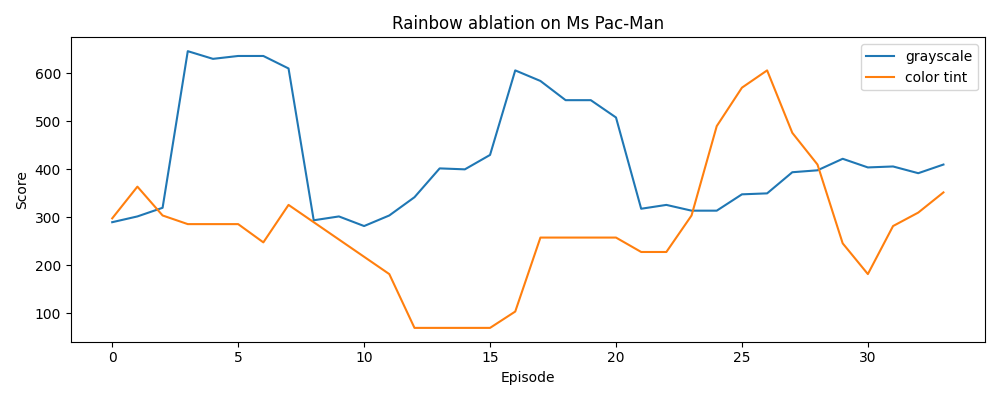
\includegraphics[width=\linewidth]{color_robustness.png}
%     \caption{Performance of Rainbow DQN under color perturbation. The model was trained on grayscale frames and evaluated in a color-tinted environment without further training.}
%     \label{fig:color_robustness}
% \end{figure}

% \subsubsection*{Implications}

% This experiment highlights a key limitation in vision-based RL: agents often fail to generalize across visually altered domains, even when the task dynamics are preserved. The reliance on pixel-level features makes them vulnerable to changes in texture, brightness, or color composition. Future work could explore techniques to mitigate this sensitivity, such as domain randomization, data augmentation, or contrastive representation learning to enforce invariance to such visual shifts.

\section{Conclusion}

In the \texttt{MsPacman-v0} environment, Rainbow DQN outperformed PPO in terms of peak reward and long-term potential. While both agents exhibited early learning, Rainbow’s combination of prioritized replay, multi-step returns, and noisy exploration proved more effective in sparse-reward, long-horizon scenarios, despite occasional instability.

PPO showed greater initial stability but suffered from later performance collapse, underscoring its sensitivity to on-policy sampling and hyperparameters. Rainbow's variance highlights its own limitations, yet in our frame budget, it demonstrated superior sample efficiency and strategic discovery.

Future work could enhance both agents by incorporating memory (e.g., LSTM) for improved temporal reasoning, extending training to tens of millions of frames to approach superhuman performance, and doing multiple runs per setting to mitigate training variance. These would strengthen agent robustness and further illuminate the challenges of mastering complex environments like Ms. Pac-Man.

\appendix
\section{Appendix}
\label{sec:appendix}

\subsection{PPO Hyperparameter Sweeps}
\begin{figure}[htbp]
  \centering
  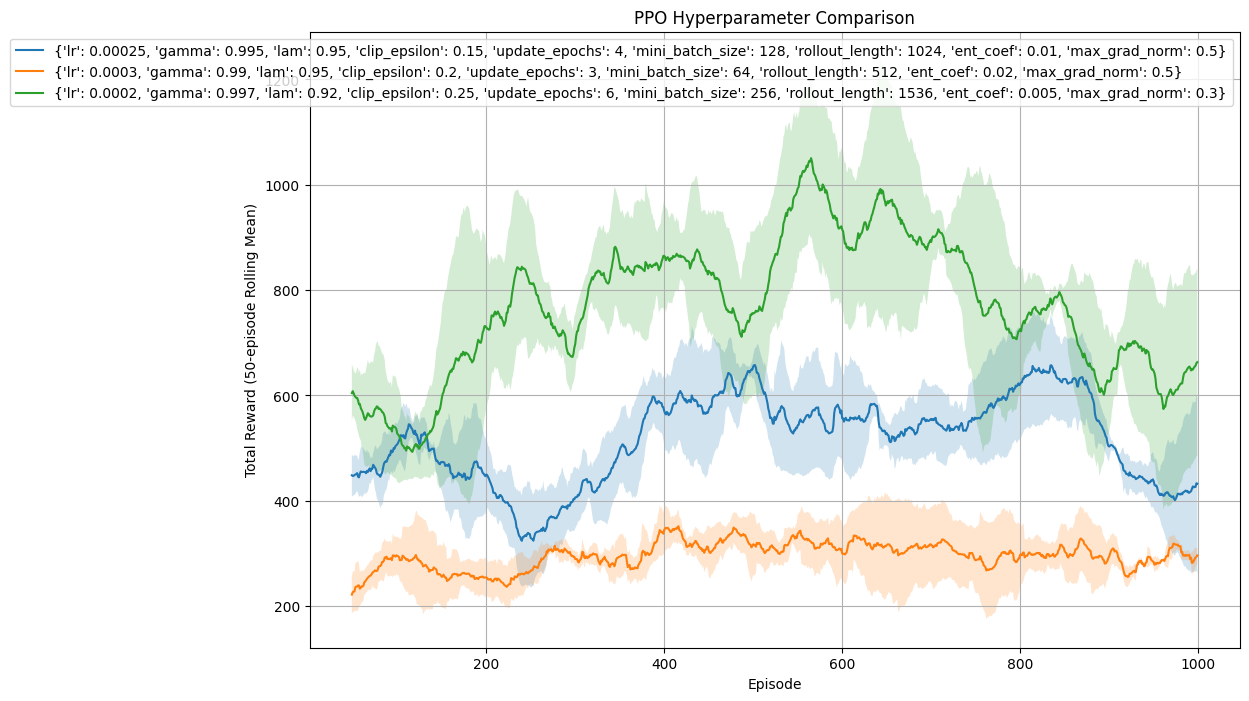
\includegraphics[width=\linewidth]{PPO_output_hyperparameters_3set.png}
  \caption{PPO Hyperparameters Optimization Results}
  \label{fig:ppo_hyperparams}
\end{figure}

\subsection{Rainbow DQN vs PPO}
\begin{figure}[htbp]
  \centering
  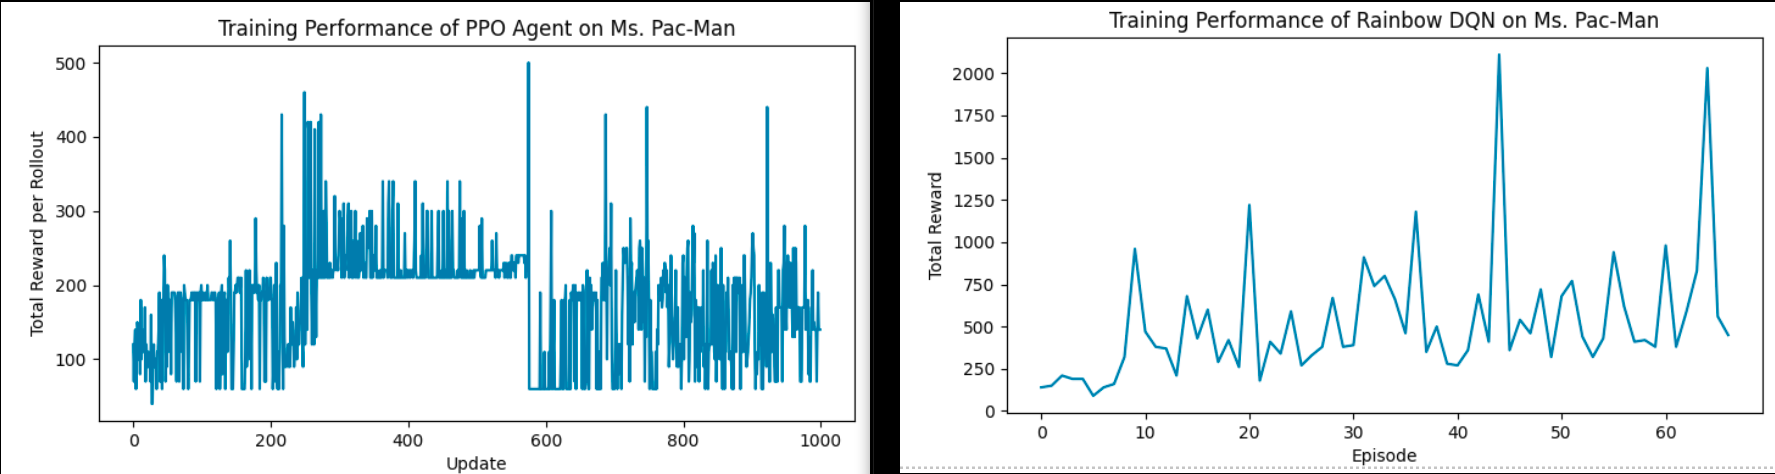
\includegraphics[width=0.85\linewidth]{rainbow_vs_ppo.png}
  \caption{Training performance of PPO and Rainbow DQN agents.}
  \label{fig:ppo_vs_rainbow}
\end{figure}

\subsection{Rainbow DQN Ablation Results}
\begin{figure}[htbp]
  \centering
  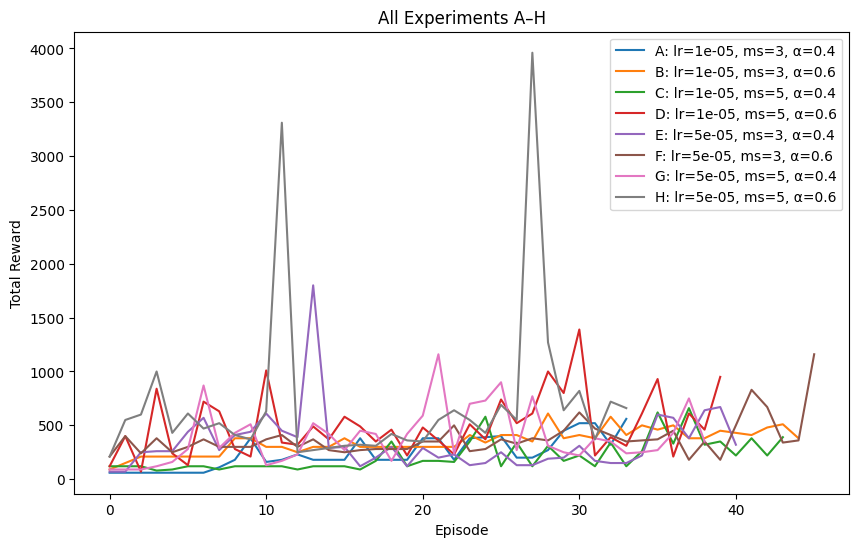
\includegraphics[width=0.8\linewidth]{rainbow_8Regular.png}
  \caption{Learning curves for the eight hyperparameter configurations:
           \(\eta\in\{1\times10^{-5},5\times10^{-5}\}\), 
           \(n\in\{3,5\}\), 
           \(\alpha\in\{0.4,0.6\}\).}
  \label{fig:ablation}
\end{figure}

\subsection{Extended Hyperparameter Sweep}
\begin{figure}[htbp]
  \centering
  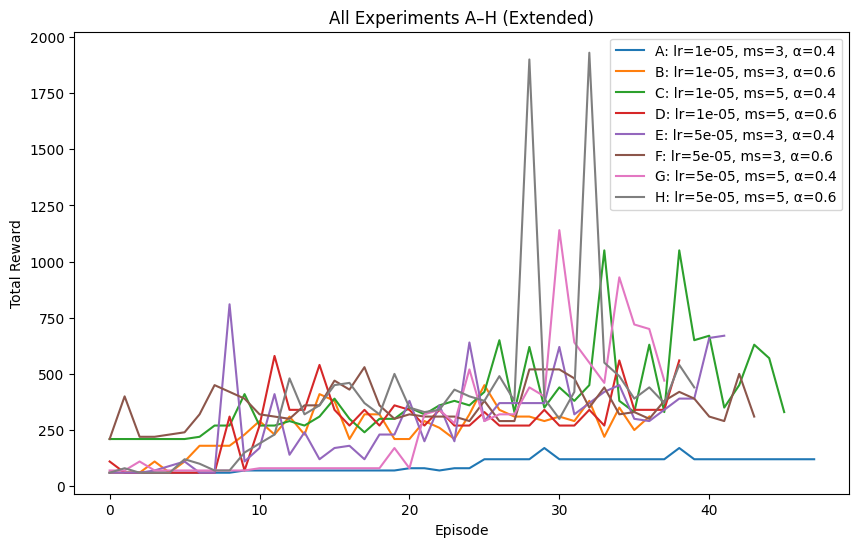
\includegraphics[width=0.9\linewidth]{rainbow_8Extended.png}
  \caption{Learning curves for the eight “large” hyperparameter runs (A\_large–H\_large).}
  \label{fig:extended_sweep}
\end{figure}

\subsection{Seed-Level Reproducibility}
\begin{figure}[htbp]
  \centering
  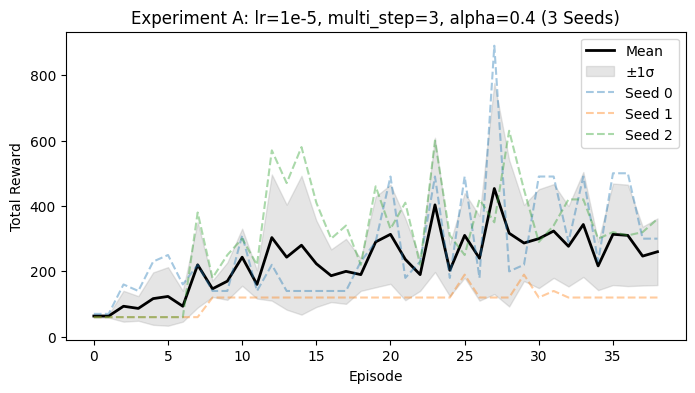
\includegraphics[width=0.8\linewidth]{rainbow_A_seed.png}
  \caption{Configuration A (\(\eta=1\times10^{-5},\,n=3,\,\alpha=0.4\)) across three seeds.}
  \label{fig:seed_A}
\end{figure}

\begin{figure}[htbp]
  \centering
  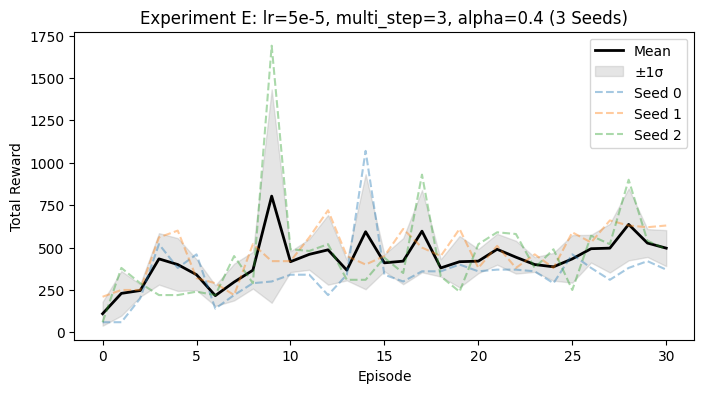
\includegraphics[width=0.8\linewidth]{rainbow_E_Seed.png}
  \caption{Configuration E (\(\eta=5\times10^{-5},\,n=3,\,\alpha=0.4\)) across three seeds.}
  \label{fig:seed_E}
\end{figure}

\subsection{Ablated Rainbow DQN Variants}
\begin{figure}[htbp]
  \centering
  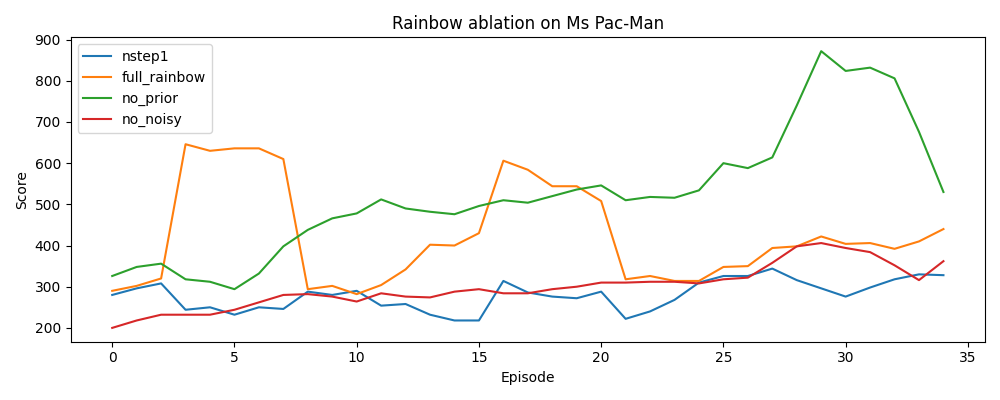
\includegraphics[width=\linewidth]{rainbow_ablation_smooth.png}
  \caption{Training performance of Rainbow DQN and ablated variants on Ms. Pac-Man.}
  \label{fig:rainbow_ablation}
\end{figure}

\clearpage
\addcontentsline{toc}{section}{References}
\bibliographystyle{plain}
\bibliography{references}

\end{document}
